\documentclass[12pt]{standalone}
\usepackage{tikz}
\usetikzlibrary{calc, patterns} % , arrows.meta, decorations.pathreplacing}

\begin{document}


\newcommand{\myy}{3.7}
		\newcommand{\ybase}{1.0}
		
		%lwarp%\begin{lateximage}[rectangles covering a horizontal line inside the square X times Y][][width: 50\%;]
		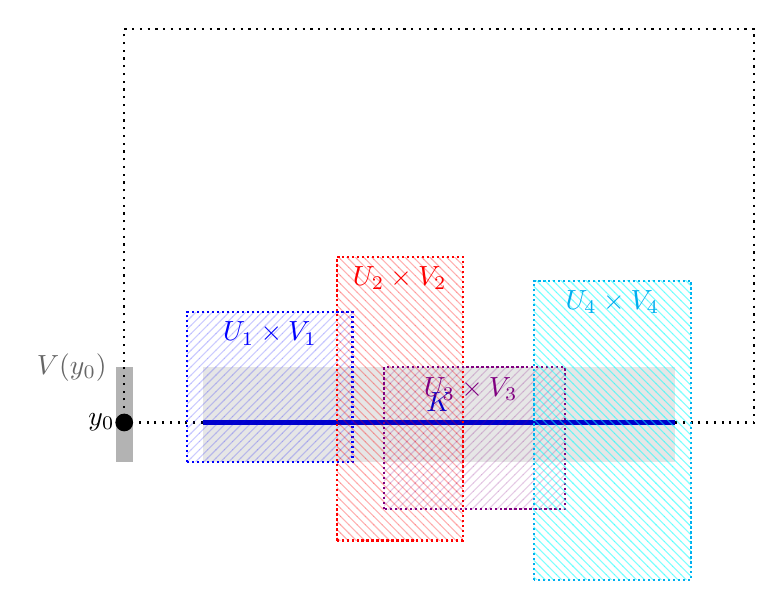
\begin{tikzpicture}
			
			\coordinate (P) at (0,\myy);
			
			\fill[gray, opacity=0.2] ($(P)+ (0,-0.5)$) rectangle ($(P)+(6,0.7)$);
			
			\draw[gray, line width=6pt, opacity=0.6] ($(P)+(-1,0)+(0,-0.5)$) -- ($(P)+(-1,0)+(0,0.7)$) node[gray!80!black, opacity=1.0, anchor=east] {$V(y_0)$};
			
			\draw[ultra thick, blue!80!black] (0,\myy) -- ++(6,0);
			
			%			% Draw x and y axes
			%			\draw[->] (0,\ybase) -- (6.5,\ybase); % node[anchor=north] {$x$};
			%			\draw[->] (0,\ybase) -- (0,6.5); % node[anchor=west] {$y$};
			%			
			\draw[ultra thick, blue!80!black] (0,\ybase) -- (6,\ybase) node[midway, anchor=south]{$K$};
			
			\draw[dotted, thick] (0, \ybase) -- (-1,\ybase) -- (-1,6) -- (7,6) -- (7, \ybase) -- (6, \ybase); 
			%\draw (0,6) -- (6,6) -- (6,\ybase);
			
			\path[save path=\Uone] ($(P) +(-0.2,-0.5)$) rectangle ++(2.1,1.9);
			\draw[thick, densely dotted, blue, use path=\Uone];
			\fill[pattern=north east lines, pattern color=blue, opacity=0.2, use path=\Uone];
			\node[anchor=north, blue] at ($(P) +(0.85,1.4)$) {$U_1\times V_1$};
			
			\path[save path=\Utwo]  ($(P) +(1.7,-1.5)$) rectangle ++(1.6,3.6);
			\draw[thick, densely dotted, red, use path=\Utwo];
			\fill[pattern=north west lines, pattern color=red, opacity=0.3, use path=\Utwo];
			\node[anchor=north, red] at ($(P) +(2.5,2.1)$) {$U_2\times V_2$};
			
			\path[save path=\Uthree]  ($(P) +(2.3,-1.1)$) rectangle ++(2.3,1.8);
			\draw[thick, densely dotted, violet, use path=\Uthree];
			\fill[pattern=north east lines, pattern color=violet, opacity=0.2, use path=\Uthree];
			\node[anchor=north, violet] at ($(P)+(3.4,0.7)$) {$U_3\times V_3$};
			
			\path[save path=\Ufour]  ($(P) +(4.2,-2.0)$) rectangle ++(2.0,3.8);
			\draw[thick, densely dotted, cyan, use path=\Ufour];
			\fill[pattern=north west lines, pattern color=cyan, opacity=0.5, use path=\Ufour];
			\node[anchor=north, cyan] at ($(P) +(5.2,1.8)$) {$U_4\times V_4$};
			
			\filldraw ($(P)+(-1,0)$) circle(3pt) node[anchor=east]{$y_0$};
			
		\end{tikzpicture}
\end{document}
